%
% file: localoperator.tex
% author: Victor Brena
% description: Briefly describes properties of the local operator.
%

\chapter{Appendix B: Issuer matched Dataset Analysis}
\label{app:app02}

%%%%%%%%%%%%%%%%%%%%%%%%%%%%%%%%%%%%%%%%%%%%%%%%%%%%%%%%%%%%
\section{B.1 Descriptive Statistics}
%%%%%%%%%%%%%%%%%%%%%%%%%%%%%%%%%%%%%%%%%%%%%%%%%%%%%%%%%%%%


%%%%%%%%%%%%%%%%%%%%%%%%%%%%%%%%%%%%%%%%%%%%%%%%%%%%%%%%%%%%
\subsection{B.1.1 Summary Statistics}
%%%%%%%%%%%%%%%%%%%%%%%%%%%%%%%%%%%%%%%%%%%%%%%%%%%%%%%%%%%%


%%%%%%%%%%%%%%%%%%%%%%%%%%%%%%%%%%%%%%%%%%%%%%%%%%%%%%%%%%%%
%\subsubsection{B.1.1.1 Green Bonds}
%%%%%%%%%%%%%%%%%%%%%%%%%%%%%%%%%%%%%%%%%%%%%%%%%%%%%%%%%%%%
\begin{table}[!htbp] \centering 
  \footnotesize
  \caption{Data Matched Green Bond Summary Statistics} 
  \label{desc2} 
\begin{tabular}{@{\extracolsep{5pt}}lccccccc} 
\\[-1.8ex]\hline 
\hline \\[-1.8ex] 
Statistic & \multicolumn{1}{c}{N} & \multicolumn{1}{c}{Mean} & \multicolumn{1}{c}{St. Dev.} & \multicolumn{1}{c}{Min} & \multicolumn{1}{c}{Pctl(25)} & \multicolumn{1}{c}{Pctl(75)} & \multicolumn{1}{c}{Max} \\ 
\hline \\[-1.8ex] 
Time to Maturity (Days) & 740 & 2,921.549 & 1,897.858 & 367 & 1,833 & 3,659 & 18,269 \\ 
Issue Amount & 740 & 1,383.033 & 2,127.100 & 500.000 & 578.613 & 1,219.467 & 33,563.640 \\ 
Coupon Rate & 740 & 1.265 & 1.196 & 0.000 & 0.375 & 1.875 & 9.500 \\ 
Guarantor & 740 & 0.143 & 0.351 & 0 & 0 & 0 & 1 \\ 
Offer Yield to Maturity & 740 & 1.301 & 1.204 & $-$0.403 & 0.420 & 1.906 & 9.500 \\
Green Flag & 740 & 1.000 & 0.000 & 1 & 1 & 1 & 1 \\ 
2008 & 740 & 0.000 & 0.000 & 0 & 0 & 0 & 0 \\ 
2009 & 740 & 0.000 & 0.000 & 0 & 0 & 0 & 0 \\ 
2010 & 740 & 0.000 & 0.000 & 0 & 0 & 0 & 0 \\ 
2011 & 740 & 0.000 & 0.000 & 0 & 0 & 0 & 0 \\ 
2012 & 740 & 0.001 & 0.037 & 0 & 0 & 0 & 1 \\ 
2013 & 740 & 0.011 & 0.103 & 0 & 0 & 0 & 1 \\ 
2014 & 740 & 0.012 & 0.110 & 0 & 0 & 0 & 1 \\ 
2015 & 740 & 0.036 & 0.188 & 0 & 0 & 0 & 1 \\ 
2016 & 740 & 0.046 & 0.210 & 0 & 0 & 0 & 1 \\ 
2017 & 740 & 0.073 & 0.260 & 0 & 0 & 0 & 1 \\ 
2018 & 740 & 0.085 & 0.279 & 0 & 0 & 0 & 1 \\ 
2019 & 740 & 0.127 & 0.333 & 0 & 0 & 0 & 1 \\ 
2020 & 740 & 0.170 & 0.376 & 0 & 0 & 0 & 1 \\ 
2021 & 740 & 0.247 & 0.432 & 0 & 0 & 0 & 1 \\ 
2022 & 740 & 0.191 & 0.393 & 0 & 0 & 0 & 1 \\ 
AAA & 740 & 0.341 & 0.474 & 0 & 0 & 1 & 1 \\ 
AA & 740 & 0.207 & 0.405 & 0 & 0 & 0 & 1 \\ 
A & 740 & 0.227 & 0.419 & 0 & 0 & 0 & 1 \\ 
BBB & 740 & 0.211 & 0.408 & 0 & 0 & 0 & 1 \\ 
BB & 740 & 0.012 & 0.110 & 0 & 0 & 0 & 1 \\ 
B & 740 & 0.003 & 0.052 & 0 & 0 & 0 & 1 \\ 
Annual Coupon & 740 & 0.682 & 0.466 & 0 & 0 & 1 & 1 \\ 
Semi Annual Coupon & 740 & 0.316 & 0.465 & 0 & 0 & 1 & 1 \\ 
Quarterly & 740 & 0.000 & 0.000 & 0 & 0 & 0 & 0 \\ 
Maturity & 740 & 0.001 & 0.037 & 0 & 0 & 0 & 1 \\ 
Basic Materials & 740 & 0.014 & 0.116 & 0 & 0 & 0 & 1 \\ 
Consumer Cyclicals & 740 & 0.008 & 0.090 & 0 & 0 & 0 & 1 \\ 
Consumer Non-Cyclicals & 740 & 0.008 & 0.090 & 0 & 0 & 0 & 1 \\ 
\hline \\[-1.8ex] 
\end{tabular} 
\end{table}

\begin{table}[!htbp] \centering 
  \footnotesize
  \caption{Data Matched Green Bond Summary Statistics cont.} 
  \label{} 
\begin{tabular}{@{\extracolsep{5pt}}lccccccc} 
\\[-1.8ex]\hline 
\hline \\[-1.8ex] 
Statistic & \multicolumn{1}{c}{N} & \multicolumn{1}{c}{Mean} & \multicolumn{1}{c}{St. Dev.} & \multicolumn{1}{c}{Min} & \multicolumn{1}{c}{Pctl(25)} & \multicolumn{1}{c}{Pctl(75)} & \multicolumn{1}{c}{Max} \\ 
\hline \\[-1.8ex] 
Energy & 740 & 0.003 & 0.052 & 0 & 0 & 0 & 1 \\ 
Financials & 740 & 0.569 & 0.496 & 0 & 0 & 1 & 1 \\ 
Government Activity & 740 & 0.195 & 0.396 & 0 & 0 & 0 & 1 \\ 
Healthcare & 740 & 0.003 & 0.052 & 0 & 0 & 0 & 1 \\ 
Industrials & 740 & 0.045 & 0.207 & 0 & 0 & 0 & 1 \\ 
Institutions, Associations \& Organizations & 740 & 0.084 & 0.277 & 0 & 0 & 0 & 1 \\ 
Real Estate & 740 & 0.018 & 0.131 & 0 & 0 & 0 & 1 \\ 
Technology & 740 & 0.009 & 0.097 & 0 & 0 & 0 & 1 \\ 
Utilities & 740 & 0.046 & 0.210 & 0 & 0 & 0 & 1 \\ 
AUD & 740 & 0.004 & 0.064 & 0 & 0 & 0 & 1 \\ 
CAD & 740 & 0.026 & 0.158 & 0 & 0 & 0 & 1 \\ 
CLP & 740 & 0.001 & 0.037 & 0 & 0 & 0 & 1 \\ 
CNY & 740 & 0.001 & 0.037 & 0 & 0 & 0 & 1 \\ 
EUR & 740 & 0.618 & 0.486 & 0 & 0 & 1 & 1 \\ 
GBP & 740 & 0.030 & 0.170 & 0 & 0 & 0 & 1 \\ 
HKD & 740 & 0.001 & 0.037 & 0 & 0 & 0 & 1 \\ 
JPY & 740 & 0.018 & 0.131 & 0 & 0 & 0 & 1 \\ 
NZD & 740 & 0.003 & 0.052 & 0 & 0 & 0 & 1 \\ 
NOK & 740 & 0.001 & 0.037 & 0 & 0 & 0 & 1 \\ 
SEK & 740 & 0.012 & 0.110 & 0 & 0 & 0 & 1 \\ 
USD & 740 & 0.284 & 0.451 & 0 & 0 & 1 & 1 \\ 
UYU & 740 & 0.001 & 0.037 & 0 & 0 & 0 & 1 \\ 
Senior Secured Mortgage & 740 & 0.064 & 0.244 & 0 & 0 & 0 & 1 \\ 
Senior Secured & 740 & 0.036 & 0.188 & 0 & 0 & 0 & 1 \\ 
Senior Unsecured & 740 & 0.732 & 0.443 & 0 & 0 & 1 & 1 \\ 
Senior Non-Preferred & 740 & 0.057 & 0.232 & 0 & 0 & 0 & 1 \\ 
Senior Preferred & 740 & 0.069 & 0.253 & 0 & 0 & 0 & 1 \\ 
Senior Subordinated Unsecured & 740 & 0.001 & 0.037 & 0 & 0 & 0 & 1 \\ 
Subordinated Unsecured & 740 & 0.007 & 0.082 & 0 & 0 & 0 & 1 \\ 
Unsecured & 740 & 0.032 & 0.177 & 0 & 0 & 0 & 1 \\ 
Public Sector & 740 & 0.482 & 0.500 & 0 & 0 & 1 & 1 \\ 
Corporate Sector & 740 & 0.518 & 0.500 & 0 & 0 & 1 & 1 \\ 
\hline \\[-1.8ex] 
\end{tabular} 
\end{table}

%%%%%%%%%%%%%%%%%%%%%%%%%%%%%%%%%%%%%%%%%%%%%%%%%%%%%%%%%%%%
%\subsubsection{B.1.1.2 Brown Bonds}
%%%%%%%%%%%%%%%%%%%%%%%%%%%%%%%%%%%%%%%%%%%%%%%%%%%%%%%%%%%%
\begin{table}[!htbp] \centering 
  \footnotesize
  \caption{Data Matched Brown Bond Summary Statistics} 
  \label{} 
\begin{tabular}{@{\extracolsep{5pt}}lccccccc} 
\\[-1.8ex]\hline 
\hline \\[-1.8ex] 
Statistic & \multicolumn{1}{c}{N} & \multicolumn{1}{c}{Mean} & \multicolumn{1}{c}{St. Dev.} & \multicolumn{1}{c}{Min} & \multicolumn{1}{c}{Pctl(25)} & \multicolumn{1}{c}{Pctl(75)} & \multicolumn{1}{c}{Max} \\ 
\hline \\[-1.8ex] 
Time to Maturity (Days) & 4,988 & 2,743.163 & 2,594.663 & 373 & 1,744.8 & 3,630.2 & 36,532 \\ 
Issue Amount & 4,988 & 1,610.370 & 1,534.290 & 500.000 & 750.000 & 1,750.000 & 30,089.370 \\ 
Coupon Rate & 4,988 & 2.160 & 1.618 & 0.001 & 0.875 & 3.125 & 20.000 \\ 
Guarantor & 4,988 & 0.186 & 0.389 & 0 & 0 & 0 & 1 \\ 
Offer Yield to Maturity & 4,988 & 2.189 & 1.623 & 0.001 & 0.940 & 3.126 & 20.000 \\
Green Flag & 4,988 & 0.000 & 0.000 & 0 & 0 & 0 & 0 \\ 
2008 & 4,988 & 0.046 & 0.210 & 0 & 0 & 0 & 1 \\ 
2009 & 4,988 & 0.057 & 0.231 & 0 & 0 & 0 & 1 \\ 
2010 & 4,988 & 0.069 & 0.254 & 0 & 0 & 0 & 1 \\ 
2011 & 4,988 & 0.074 & 0.261 & 0 & 0 & 0 & 1 \\
2012 & 4,988 & 0.090 & 0.287 & 0 & 0 & 0 & 1 \\ 
2013 & 4,988 & 0.075 & 0.263 & 0 & 0 & 0 & 1 \\ 
2014 & 4,988 & 0.076 & 0.265 & 0 & 0 & 0 & 1 \\ 
\hline \\[-1.8ex] 
\end{tabular} 
\end{table} 

\newpage

\begin{table}[!ht] \centering 
  \footnotesize
  \caption{Data Matched Brown Bond Summary Statistics cont.} 
  \label{} 
\begin{tabular}{@{\extracolsep{5pt}}lccccccc} 
\\[-1.8ex]\hline 
\hline \\[-1.8ex] 
Statistic & \multicolumn{1}{c}{N} & \multicolumn{1}{c}{Mean} & \multicolumn{1}{c}{St. Dev.} & \multicolumn{1}{c}{Min} & \multicolumn{1}{c}{Pctl(25)} & \multicolumn{1}{c}{Pctl(75)} & \multicolumn{1}{c}{Max} \\ 
\hline \\[-1.8ex]
2015 & 4,988 & 0.081 & 0.273 & 0 & 0 & 0 & 1 \\ 
2016 & 4,988 & 0.082 & 0.275 & 0 & 0 & 0 & 1 \\ 
2017 & 4,988 & 0.071 & 0.257 & 0 & 0 & 0 & 1 \\ 
2018 & 4,988 & 0.068 & 0.251 & 0 & 0 & 0 & 1 \\ 
2019 & 4,988 & 0.073 & 0.260 & 0 & 0 & 0 & 1 \\ 
2020 & 4,988 & 0.051 & 0.219 & 0 & 0 & 0 & 1 \\ 
2021 & 4,988 & 0.042 & 0.200 & 0 & 0 & 0 & 1 \\ 
2022 & 4,988 & 0.046 & 0.209 & 0 & 0 & 0 & 1 \\ 
AAA & 4,988 & 0.450 & 0.498 & 0 & 0 & 1 & 1 \\ 
AA & 4,988 & 0.270 & 0.444 & 0 & 0 & 1 & 1 \\ 
A & 4,988 & 0.139 & 0.346 & 0 & 0 & 0 & 1 \\ 
BBB & 4,988 & 0.127 & 0.333 & 0 & 0 & 0 & 1 \\ 
BB & 4,988 & 0.012 & 0.108 & 0 & 0 & 0 & 1 \\ 
B & 4,988 & 0.002 & 0.045 & 0 & 0 & 0 & 1 \\ 
Annual Coupon & 4,988 & 0.631 & 0.483 & 0 & 0 & 1 & 1 \\ 
Semi Annual Coupon & 4,988 & 0.366 & 0.482 & 0 & 0 & 1 & 1 \\ 
Quarterly & 4,988 & 0.002 & 0.047 & 0 & 0 & 0 & 1 \\ 
Maturity & 4,988 & 0.001 & 0.028 & 0 & 0 & 0 & 1 \\ 
Basic Materials & 4,988 & 0.005 & 0.071 & 0 & 0 & 0 & 1 \\ 
Consumer Cyclicals & 4,988 & 0.006 & 0.077 & 0 & 0 & 0 & 1 \\ 
Consumer Non-Cyclicals & 4,988 & 0.002 & 0.049 & 0 & 0 & 0 & 1 \\ 
Energy & 4,988 & 0.005 & 0.072 & 0 & 0 & 0 & 1 \\ 
Financials & 4,988 & 0.675 & 0.469 & 0 & 0 & 1 & 1 \\ 
Government Activity & 4,988 & 0.233 & 0.423 & 0 & 0 & 0 & 1 \\ 
Healthcare & 4,988 & 0.001 & 0.028 & 0 & 0 & 0 & 1 \\ 
Industrials & 4,988 & 0.011 & 0.106 & 0 & 0 & 0 & 1 \\ 
Institutions, Associations \& Organizations & 4,988 & 0.038 & 0.192 & 0 & 0 & 0 & 1 \\ 
Real Estate & 4,988 & 0.001 & 0.028 & 0 & 0 & 0 & 1 \\ 
Technology & 4,988 & 0.008 & 0.087 & 0 & 0 & 0 & 1 \\ 
Utilities & 4,988 & 0.014 & 0.118 & 0 & 0 & 0 & 1 \\ 
AUD & 4,988 & 0.014 & 0.118 & 0 & 0 & 0 & 1 \\ 
CAD & 4,988 & 0.004 & 0.066 & 0 & 0 & 0 & 1 \\ 
CLP & 4,988 & 0.0004 & 0.020 & 0 & 0 & 0 & 1 \\ 
CNY & 4,988 & 0.0002 & 0.014 & 0 & 0 & 0 & 1 \\ 
EUR & 4,988 & 0.528 & 0.499 & 0 & 0 & 1 & 1 \\ 
GBP & 4,988 & 0.062 & 0.242 & 0 & 0 & 0 & 1 \\ 
HKD & 4,988 & 0.0002 & 0.014 & 0 & 0 & 0 & 1 \\ 
JPY & 4,988 & 0.021 & 0.145 & 0 & 0 & 0 & 1 \\ 
NZD & 4,988 & 0.001 & 0.028 & 0 & 0 & 0 & 1 \\ 
NOK & 4,988 & 0.0004 & 0.020 & 0 & 0 & 0 & 1 \\ 
SEK & 4,988 & 0.0002 & 0.014 & 0 & 0 & 0 & 1 \\ 
USD & 4,988 & 0.364 & 0.481 & 0 & 0 & 1 & 1 \\ 
UYU & 4,988 & 0.0004 & 0.020 & 0 & 0 & 0 & 1 \\ 
Senior Secured Mortgage & 4,988 & 0.088 & 0.284 & 0 & 0 & 0 & 1 \\ 
Senior Secured & 4,988 & 0.059 & 0.235 & 0 & 0 & 0 & 1 \\ 
Senior Unsecured & 4,988 & 0.647 & 0.478 & 0 & 0 & 1 & 1 \\ 
Senior Non-Preferred & 4,988 & 0.029 & 0.167 & 0 & 0 & 0 & 1 \\ 
Senior Preferred & 4,988 & 0.048 & 0.214 & 0 & 0 & 0 & 1 \\ 
Senior Subordinated Unsecured & 4,988 & 0.002 & 0.049 & 0 & 0 & 0 & 1 \\ 
Subordinated Unsecured & 4,988 & 0.020 & 0.141 & 0 & 0 & 0 & 1 \\ 
Unsecured & 4,988 & 0.090 & 0.286 & 0 & 0 & 0 & 1 \\ 
Public Sector & 4,988 & 0.504 & 0.500 & 0 & 0 & 1 & 1 \\ 
Corporate Sector & 4,988 & 0.496 & 0.500 & 0 & 0 & 1 & 1 \\ 
\hline \\[-1.8ex] 
\end{tabular} 
\end{table} 

\newpage

%%%%%%%%%%%%%%%%%%%%%%%%%%%%%%%%%%%%%%%%%%%%%%%%%%%%%%%%%%%%
\subsection{B.1.2 Raincloud Plots}
%%%%%%%%%%%%%%%%%%%%%%%%%%%%%%%%%%%%%%%%%%%%%%%%%%%%%%%%%%%%

\begin{figure}[h!]
    \centering
    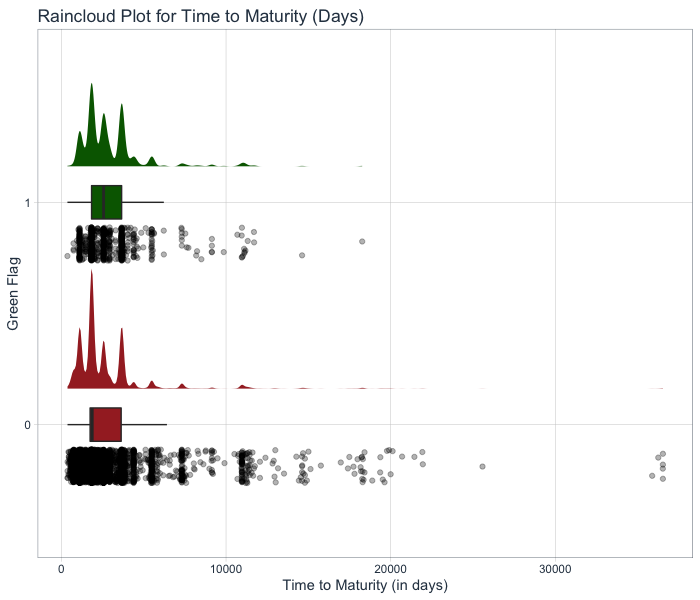
\includegraphics[scale=0.45]{chinchilab-template/chapters/appendices/ANALYSIS/raincloud2_ttm.png}
    \caption{Raincloud Plot for Time to Maturity (Days)}
    \label{fig:my_label}
\end{figure}

\begin{figure}[h!]
    \centering
    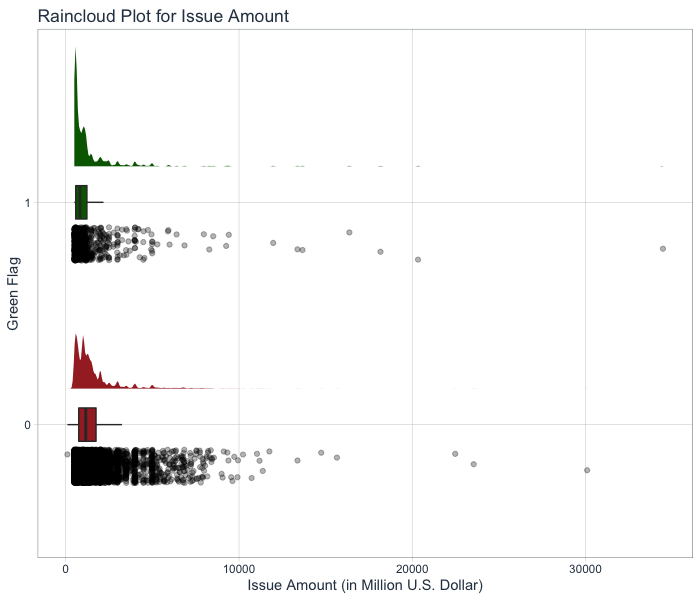
\includegraphics[scale=0.45]{chinchilab-template/chapters/appendices/ANALYSIS/raincloud2_size.png}
    \caption{Raincloud for Issue Amount}
    \label{fig:my_label}
\end{figure}

\begin{figure}[h!]
    \centering
    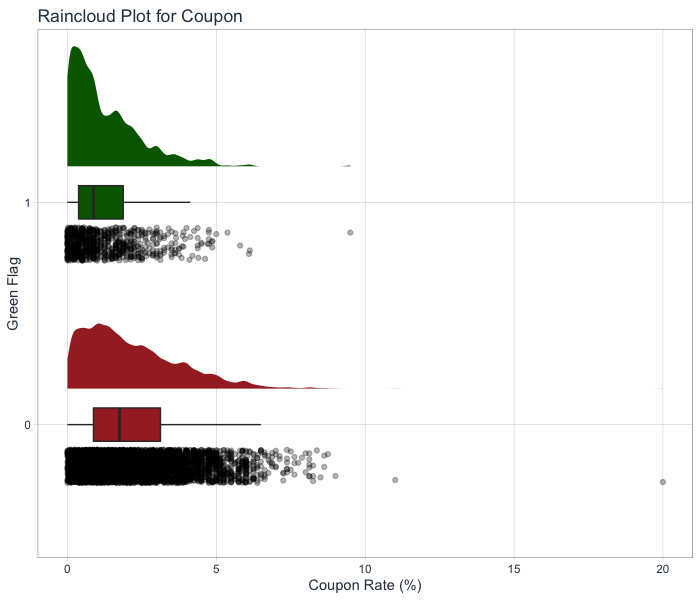
\includegraphics[scale=0.47]{chinchilab-template/chapters/appendices/ANALYSIS/raincloud2_coupon.png}
    \caption{Raincloud for Coupon Rate}
    \label{fig:my_label}
\end{figure}

\begin{figure}[h!]
    \centering
    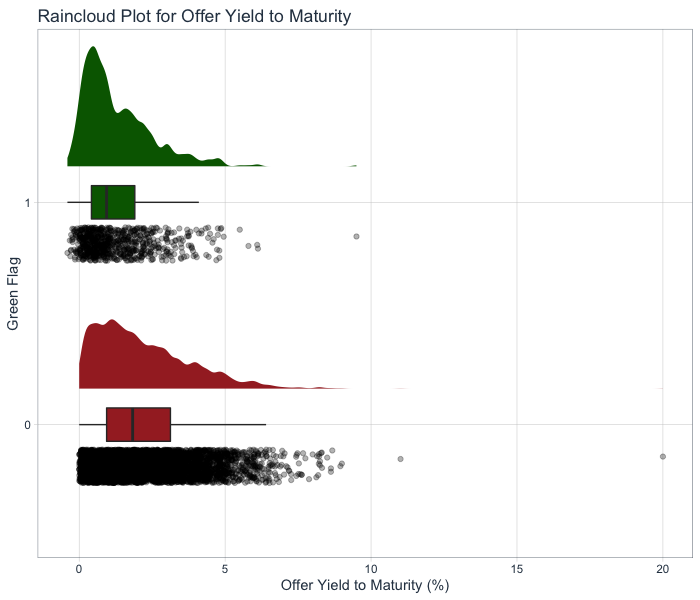
\includegraphics[scale=0.47]{chinchilab-template/chapters/appendices/ANALYSIS/raincloud2_ytm.png}
    \caption{Raincloud for Issuance Yield}
    \label{fig:my_label}
\end{figure}

\newpage

%%%%%%%%%%%%%%%%%%%%%%%%%%%%%%%%%%%%%%%%%%%%%%%%%%%%%%%%%%%%
\subsection{B.1.3 Correlation}
%%%%%%%%%%%%%%%%%%%%%%%%%%%%%%%%%%%%%%%%%%%%%%%%%%%%%%%%%%%%

\begin{figure}[h!]
    \centering
    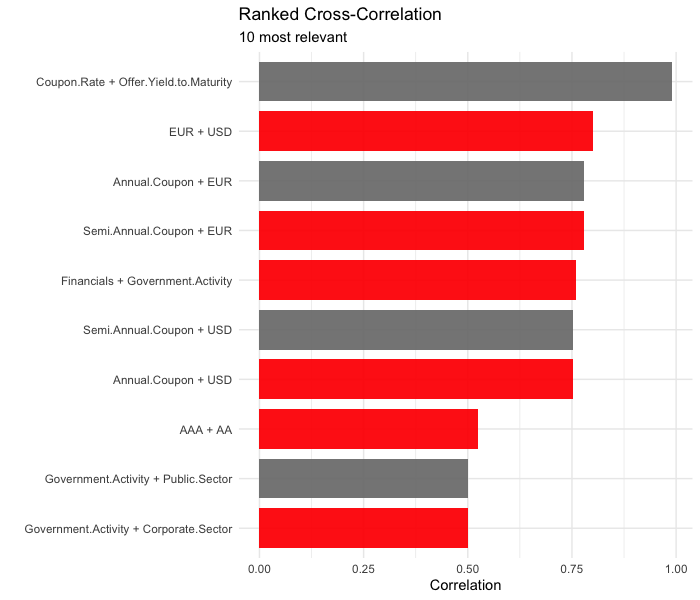
\includegraphics[scale=0.45]{chinchilab-template/chapters/appendices/ANALYSIS/correlation2.png}
    \caption{Ranked Cross-Correlation of 10 Most Relevant Pairs}
    \caption*{Note: Blue = Positive Correlation, Red = Negative Correlation.}
    \label{fig:my_label}
\end{figure}

%%%%%%%%%%%%%%%%%%%%%%%%%%%%%%%%%%%%%%%%%%%%%%%%%%%%%%%%%%%%
\subsection{B.1.4 Propensity Tables}
%%%%%%%%%%%%%%%%%%%%%%%%%%%%%%%%%%%%%%%%%%%%%%%%%%%%%%%%%%%%

\begin{table}[H]{
    \begin{subtable}{.5\textwidth}
    \footnotesize
    \centering
        {\begin{tabular}{lll}
        \\[-1.8ex]\hline 
        \hline \\[-1.8ex] 
        \textbf{Issue Year} & \textbf{Green (\%)} & \textbf{Brown (\%)} \\
        \hline \\[-1.8ex]
        {\color[HTML]{333333} 2008} & \cellcolor[HTML]{FFFFFF}{\color[HTML]{333333} 0.0} & \cellcolor[HTML]{EBF2E9}{\color[HTML]{333333} 4.6} \\
        \cellcolor[HTML]{FAFAFA}{\color[HTML]{333333} 2009} & \cellcolor[HTML]{FFFFFF}{\color[HTML]{333333} 0.0} & \cellcolor[HTML]{B6CDAE}{\color[HTML]{333333} 5.7} \\
        {\color[HTML]{333333} 2010} & \cellcolor[HTML]{FFFFFF}{\color[HTML]{333333} 0.0} & \cellcolor[HTML]{7DA670}{\color[HTML]{333333} 6.9} \\
        \cellcolor[HTML]{FAFAFA}{\color[HTML]{333333} 2011} & \cellcolor[HTML]{FFFFFF}{\color[HTML]{333333} 0.0} & \cellcolor[HTML]{659658}{\color[HTML]{333333} 7.4} \\
        {\color[HTML]{333333} 2012} & \cellcolor[HTML]{FEFEFE}{\color[HTML]{333333} 0.1} & \cellcolor[HTML]{006400}{\color[HTML]{FFFFFF} 9.0} \\
        \cellcolor[HTML]{FAFAFA}{\color[HTML]{333333} 2013} & \cellcolor[HTML]{F4F8F3}{\color[HTML]{333333} 1.1} & \cellcolor[HTML]{619353}{\color[HTML]{FFFFFF} 7.5} \\
        {\color[HTML]{333333} 2014} & \cellcolor[HTML]{F4F7F2}{\color[HTML]{333333} 1.2} & \cellcolor[HTML]{5C904E}{\color[HTML]{FFFFFF} 7.6} \\
        \cellcolor[HTML]{FAFAFA}{\color[HTML]{333333} 2015} & \cellcolor[HTML]{DDE8D9}{\color[HTML]{333333} 3.6} & \cellcolor[HTML]{438035}{\color[HTML]{FFFFFF} 8.1} \\
        {\color[HTML]{333333} 2016} & \cellcolor[HTML]{D3E1CE}{\color[HTML]{333333} 4.6} & \cellcolor[HTML]{3D7D30}{\color[HTML]{FFFFFF} 8.2} \\
        \cellcolor[HTML]{FAFAFA}{\color[HTML]{333333} 2017} & \cellcolor[HTML]{BAD0B2}{\color[HTML]{333333} 7.3} & \cellcolor[HTML]{74A066}{\color[HTML]{333333} 7.1} \\
        {\color[HTML]{333333} 2018} & \cellcolor[HTML]{AFC8A6}{\color[HTML]{333333} 8.5} & \cellcolor[HTML]{82AA75}{\color[HTML]{333333} 6.8} \\
        \cellcolor[HTML]{FAFAFA}{\color[HTML]{333333} 2019} & \cellcolor[HTML]{88AE7C}{\color[HTML]{333333} 12.7} & \cellcolor[HTML]{6A9A5D}{\color[HTML]{333333} 7.3} \\
        {\color[HTML]{333333} 2020} & \cellcolor[HTML]{609353}{\color[HTML]{FFFFFF} 17.0} & \cellcolor[HTML]{D3E1CE}{\color[HTML]{333333} 5.1} \\
        \cellcolor[HTML]{FAFAFA}{\color[HTML]{333333} 2021} & \cellcolor[HTML]{006400}{\color[HTML]{FFFFFF} 24.7} & \cellcolor[HTML]{FFFFFF}{\color[HTML]{333333} 4.2} \\
        {\color[HTML]{333333} 2022} & \cellcolor[HTML]{4C863F}{\color[HTML]{FFFFFF} 19.1} & \cellcolor[HTML]{EBF2E9}{\color[HTML]{333333} 4.6} \\
        \hline \\[-1.8ex]
        \end{tabular}}
    \subcaption{Issue Year}
    \label{propyear}
    \end{subtable}
    \begin{subtable}{0.3\linewidth}
    \footnotesize
    \centering
        {\begin{tabular}{lll}
        \\[-1.8ex]\hline 
        \hline \\[-1.8ex] 
        \textbf{Rating} & \textbf{Green (\%)} & \textbf{Brown (\%)} \\
        \hline \\[-1.8ex]
        \rowcolor[HTML]{006400} 
        \cellcolor[HTML]{FFFFFF}{\color[HTML]{333333} AAA} & {\color[HTML]{FFFFFF} 34.1} & {\color[HTML]{FFFFFF} 45.0} \\
        \cellcolor[HTML]{FAFAFA}{\color[HTML]{333333} AA} & \cellcolor[HTML]{739F66}{\color[HTML]{333333} 20.7} & \cellcolor[HTML]{75A167}{\color[HTML]{333333} 27.0} \\
        \cellcolor[HTML]{FFFFFF}{\color[HTML]{333333} A} & \cellcolor[HTML]{669658}{\color[HTML]{333333} 22.7} & \cellcolor[HTML]{B7CEAF}{\color[HTML]{333333} 13.9} \\
        \cellcolor[HTML]{FAFAFA}{\color[HTML]{333333} BBB} & \cellcolor[HTML]{709E63}{\color[HTML]{333333} 21.1} & \cellcolor[HTML]{BDD2B5}{\color[HTML]{333333} 12.7} \\
        \cellcolor[HTML]{FFFFFF}{\color[HTML]{333333} BB} & \cellcolor[HTML]{F7F9F6}{\color[HTML]{333333} 1.2} & \cellcolor[HTML]{F9FBF8}{\color[HTML]{333333} 1.2} \\
        \cellcolor[HTML]{FAFAFA}{\color[HTML]{333333} B} & \cellcolor[HTML]{FDFEFD}{\color[HTML]{333333} 0.3} & \cellcolor[HTML]{FEFEFE}{\color[HTML]{333333} 0.2} \\
        \rowcolor[HTML]{FFFFFF} 
        {\color[HTML]{333333} CCC} & {\color[HTML]{333333} 0.0} & {\color[HTML]{333333} 0.0} \\
        \hline \\[-1.8ex]
        \end{tabular}}
    \subcaption{Rating}
    \label{proprating}
    \end{subtable}
\caption{Propensity Tables}}
\end{table}

\begin{table}[h!]
\centering
\caption{Propensity Table for Coupon Frequency}
\footnotesize
\begin{tabular}{lll}
\\[-1.8ex]\hline 
\hline \\[-1.8ex] 
\cellcolor[HTML]{FFFFFF}{\color[HTML]{333333} \textbf{Coupon Frequency}} & {\color[HTML]{333333} \textbf{Green (\%)}} & {\color[HTML]{333333} \textbf{Brown (\%)}} \\
\hline \\[-1.8ex] 
\rowcolor[HTML]{006400} 
\cellcolor[HTML]{FFFFFF}{\color[HTML]{333333} Annual Coupon} & {\color[HTML]{FFFFFF} 68.2} & {\color[HTML]{FFFFFF} 63.1} \\
\cellcolor[HTML]{FAFAFA}{\color[HTML]{333333} Semi Annual Coupon} & \cellcolor[HTML]{94B688}{\color[HTML]{333333} 31.6} & \cellcolor[HTML]{79A46C}{\color[HTML]{333333} 36.6} \\
\rowcolor[HTML]{FFFFFF} 
{\color[HTML]{333333} Quarterly} & {\color[HTML]{333333} 0.0} & {\color[HTML]{333333} 0.2} \\
\rowcolor[HTML]{FFFFFF} 
\cellcolor[HTML]{FAFAFA}{\color[HTML]{333333} Maturity} & {\color[HTML]{333333} 0.1} & {\color[HTML]{333333} 0.1} \\
\hline \\[-1.8ex] 
\end{tabular}
\end{table}

\begin{table}[h!] \centering
\caption{Propensity Table for Industry}
\footnotesize
\begin{tabular}{lll}
\\[-1.8ex]\hline 
\hline \\[-1.8ex] 
\cellcolor[HTML]{FFFFFF}{\color[HTML]{333333} \textbf{TRBC Industry}} & \cellcolor[HTML]{FFFFFF}{\color[HTML]{333333} \textbf{Green (\%)}} & \cellcolor[HTML]{FFFFFF}{\color[HTML]{333333} \textbf{Brown (\%)}} \\
\hline \\[-1.8ex] 
\rowcolor[HTML]{FFFFFF} 
{\color[HTML]{333333} Academic \& Educational Services} & {\color[HTML]{333333} 0.0} & {\color[HTML]{333333} 0.0} \\
\cellcolor[HTML]{FAFAFA}{\color[HTML]{333333} Basic Materials} & \cellcolor[HTML]{F9FBF8}{\color[HTML]{333333} 1.4} & \cellcolor[HTML]{FDFEFD}{\color[HTML]{333333} 0.5} \\
\cellcolor[HTML]{FFFFFF}{\color[HTML]{333333} Consumer Cyclicals} & \cellcolor[HTML]{FCFDFB}{\color[HTML]{333333} 0.8} & \cellcolor[HTML]{FDFEFD}{\color[HTML]{333333} 0.6} \\
\cellcolor[HTML]{FAFAFA}{\color[HTML]{333333} Consumer Non-Cyclicals} & \cellcolor[HTML]{FCFDFB}{\color[HTML]{333333} 0.8} & \cellcolor[HTML]{FEFFFE}{\color[HTML]{333333} 0.2} \\
\cellcolor[HTML]{FFFFFF}{\color[HTML]{333333} Energy} & \cellcolor[HTML]{FEFEFE}{\color[HTML]{333333} 0.3} & \cellcolor[HTML]{FDFEFD}{\color[HTML]{333333} 0.5} \\
\rowcolor[HTML]{006400} 
\cellcolor[HTML]{FAFAFA}{\color[HTML]{333333} Financials} & {\color[HTML]{FFFFFF} 56.9} & {\color[HTML]{FFFFFF} 67.5} \\
\rowcolor[HTML]{AFC8A6} 
\cellcolor[HTML]{FFFFFF}{\color[HTML]{333333} Government Activity} & {\color[HTML]{333333} 19.5} & {\color[HTML]{333333} 23.3} \\
\cellcolor[HTML]{FAFAFA}{\color[HTML]{333333} Healthcare} & \cellcolor[HTML]{FEFEFE}{\color[HTML]{333333} 0.3} & \cellcolor[HTML]{FFFFFF}{\color[HTML]{333333} 0.1} \\
\cellcolor[HTML]{FFFFFF}{\color[HTML]{333333} Industrials} & \cellcolor[HTML]{ECF2EA}{\color[HTML]{333333} 4.5} & \cellcolor[HTML]{FBFCFB}{\color[HTML]{333333} 1.1} \\
\cellcolor[HTML]{FAFAFA}{\color[HTML]{333333} Institutions, Associations \& Organizations} & \cellcolor[HTML]{DCE7D8}{\color[HTML]{333333} 8.4} & \cellcolor[HTML]{F2F6F0}{\color[HTML]{333333} 3.8} \\
\rowcolor[HTML]{FFFFFF} 
{\color[HTML]{333333} Real Estate} & \cellcolor[HTML]{F8FAF7}{\color[HTML]{333333} 1.8} & {\color[HTML]{333333} 0.1} \\
\cellcolor[HTML]{FAFAFA}{\color[HTML]{333333} Technology} & \cellcolor[HTML]{FBFCFB}{\color[HTML]{333333} 0.9} & \cellcolor[HTML]{FCFDFC}{\color[HTML]{333333} 0.8} \\
\cellcolor[HTML]{FFFFFF}{\color[HTML]{333333} Utilities} & \cellcolor[HTML]{ECF2EA}{\color[HTML]{333333} 4.6} & \cellcolor[HTML]{FAFCF9}{\color[HTML]{333333} 1.4} \\
\hline \\[-1.8ex] 
\end{tabular}
\end{table}

\begin{table}[h!] \centering
\caption{Propensity Table for Currency}
\footnotesize
\begin{tabular}{llllll}
\\[-1.8ex]\hline 
\hline \\[-1.8ex] 
\textbf{Currency} & \textbf{Green (\%)} & \textbf{Brown (\%)} &  & \textbf{Green (\%)} & \textbf{Brown (\%)} \\
\hline \\[-1.8ex]
{\color[HTML]{333333} AUD} & \cellcolor[HTML]{FDFEFD}{\color[HTML]{333333} 0.4} & \cellcolor[HTML]{FBFCFA}{\color[HTML]{333333} 1.4} & {\color[HTML]{333333} NZD} & \cellcolor[HTML]{FEFEFE}{\color[HTML]{333333} 0.3} & {\color[HTML]{333333} 0.1} \\
{\color[HTML]{333333} BRL} & {\color[HTML]{333333} 0.0} & {\color[HTML]{333333} 0.0} & {\color[HTML]{333333} NOK} & {\color[HTML]{333333} 0.1} & {\color[HTML]{333333} 0.0} \\
{\color[HTML]{333333} CAD} & \cellcolor[HTML]{F7F9F5}{\color[HTML]{333333} 2.6} & \cellcolor[HTML]{FBFCFA}{\color[HTML]{333333} 0.4} & {\color[HTML]{333333} PEN} & {\color[HTML]{333333} 0.0} & {\color[HTML]{333333} 0.0} \\
{\color[HTML]{333333} CLP} & {\color[HTML]{333333} 0.1} & {\color[HTML]{333333} 0.0} & {\color[HTML]{333333} PHP} & {\color[HTML]{333333} 0.0} & {\color[HTML]{333333} 0.0} \\
{\color[HTML]{333333} CNY} & {\color[HTML]{333333} 0.1} & {\color[HTML]{333333} 0.0} & {\color[HTML]{333333} RUB} & {\color[HTML]{333333} 0.0} & {\color[HTML]{333333} 0.0} \\
{\color[HTML]{333333} COP} & {\color[HTML]{333333} 0.0} & {\color[HTML]{333333} 0.0} & {\color[HTML]{333333} SGD} & {\color[HTML]{333333} 0.0} & {\color[HTML]{333333} 0.0} \\
{\color[HTML]{333333} HRK} & {\color[HTML]{333333} 0.0} & {\color[HTML]{333333} 0.0} & {\color[HTML]{333333} SEK} & \cellcolor[HTML]{FBFCFB}{\color[HTML]{333333} 1.2} & {\color[HTML]{333333} 0.0} \\
{\color[HTML]{333333} EUR} & \cellcolor[HTML]{006400}{\color[HTML]{FFFFFF} 61.8} & \cellcolor[HTML]{006400}{\color[HTML]{FFFFFF} 52.8} & {\color[HTML]{333333} CHF} & {\color[HTML]{333333} 0.0} & \cellcolor[HTML]{FAFCFA}{\color[HTML]{333333} 0.2} \\
{\color[HTML]{333333} GBP} & \cellcolor[HTML]{F3F7F1}{\color[HTML]{333333} 3.0} & \cellcolor[HTML]{E5EDE1}{\color[HTML]{333333} 6.2} & {\color[HTML]{333333} THB} & {\color[HTML]{333333} 0.0} & {\color[HTML]{333333} 0.0} \\
{\color[HTML]{333333} HKD} & {\color[HTML]{333333} 0.1} & {\color[HTML]{333333} 0.0} & {\color[HTML]{333333} TRY} & {\color[HTML]{333333} 0.0} & {\color[HTML]{333333} 0.0} \\
{\color[HTML]{333333} JPY} & \cellcolor[HTML]{FAFCF9}{\color[HTML]{333333} 1.8} & \cellcolor[HTML]{F0F5EE}{\color[HTML]{333333} 2.1} & {\color[HTML]{333333} USD} & \cellcolor[HTML]{6B9A5E}{\color[HTML]{333333} 28.4} & \cellcolor[HTML]{3F7E32}{\color[HTML]{FFFFFF} 36.4} \\
{\color[HTML]{333333} KZT} & {\color[HTML]{333333} 0.0} & {\color[HTML]{333333} 0.0} & \cellcolor[HTML]{FFFFFF}UYU & \cellcolor[HTML]{FFFFFF}0.1 & \cellcolor[HTML]{FFFFFF}0.0 \\
\cellcolor[HTML]{FFFFFF}{\color[HTML]{333333} MXN} & {\color[HTML]{333333} 0.0} & {\color[HTML]{333333} 0.0} & \cellcolor[HTML]{FFFFFF} & \multicolumn{1}{l}{\cellcolor[HTML]{FFFFFF}} & \multicolumn{1}{l}{\cellcolor[HTML]{FFFFFF}} \\
\hline \\[-1.8ex]
\end{tabular}
\end{table}

\newpage

\begin{table}[H]{
    \begin{subtable}{.5\textwidth}
    \centering
    \footnotesize
        {\begin{tabular}{lll}
        \\[-1.8ex]\hline 
        \hline \\[-1.8ex] 
        \textbf{Issuer Sector} & \textbf{Green (\%)} & \textbf{Brown (\%)} \\
        \hline \\[-1.8ex]
        \cellcolor[HTML]{FFFFFF}{\color[HTML]{333333} Public Sector} & {\color[HTML]{333333} 48.2} & {\color[HTML]{333333} 50.4} \\
        \rowcolor[HTML]{006400} 
        \cellcolor[HTML]{FFFFFF}{\color[HTML]{333333} Corporate Sector} & {\color[HTML]{FFFFFF} 51.8} & {\color[HTML]{FFFFFF} 49.6} \\
        \\[-1.8ex]\hline 
        \end{tabular}}
    \subcaption{Issuer Sector}
    \end{subtable}
    \begin{subtable}{0.3\linewidth}
    \centering
    \footnotesize
        {\begin{tabular}{lll}
        \\[-1.8ex]\hline 
        \hline \\[-1.8ex] 
        \textbf{Guarantor} & \textbf{Green (\%)} & \textbf{Brown (\%)} \\
        \hline \\[-1.8ex]
        \rowcolor[HTML]{FFFFFF} 
        {\color[HTML]{333333} Guarantor} & {\color[HTML]{333333} 14.3} & {\color[HTML]{333333} 18.6} \\
        \rowcolor[HTML]{006400} 
        \cellcolor[HTML]{FAFAFA}{\color[HTML]{333333} No Guarantor} & {\color[HTML]{FFFFFF} 85.7} & {\color[HTML]{FFFFFF} 81.4} \\
        \hline \\[-1.8ex]
        \end{tabular}}
    \subcaption{Guarantor}
    \end{subtable}
\caption{Propensity Table for Issuer Sector and Guarantor}
\label{x}}
\end{table}

\begin{table}[H] \centering
\caption{Propensity Table for Seniority}
\footnotesize
\begin{tabular}{llllll}
\\[-1.8ex]\hline 
\hline \\[-1.8ex] 
\cellcolor[HTML]{FFFFFF}{\color[HTML]{333333} \textbf{Seniority}} & \cellcolor[HTML]{FFFFFF}{\color[HTML]{333333} \textbf{Green (\%)}} & \cellcolor[HTML]{FFFFFF}{\color[HTML]{333333} \textbf{Brown (\%)}} \\
\hline \\[-1.8ex]
First-Lien Loan & 0.0 & 0.0 \\
\cellcolor[HTML]{FAFAFA}First Mortgage & 0.0 & 0.0 \\
First Refunding Mortgage & 0.0 & 0.0 \\
\cellcolor[HTML]{FAFAFA}Second-Lien Loan & 0.0 & 0.0 \\
Junior Subordinated & 0.0 & 0.0 \\
\cellcolor[HTML]{FAFAFA}Senior Secured Mortgage & \cellcolor[HTML]{EAF1E8}6.4 & \cellcolor[HTML]{DFE9DB}8.8 \\
Refunding Mortgage & 0.0 & 0.0 \\
\cellcolor[HTML]{FAFAFA}Senior Secured & \cellcolor[HTML]{006400}{\color[HTML]{FFFFFF} 73.2} & \cellcolor[HTML]{006400}{\color[HTML]{FFFFFF} 64.7} \\
Senior Unsecured & \cellcolor[HTML]{EDF2EA}5.7 & \cellcolor[HTML]{F4F8F3}2.9 \\
\cellcolor[HTML]{FAFAFA}Senior Non-Preferred & \cellcolor[HTML]{E9F0E6}6.9 & \cellcolor[HTML]{EEF3EB}4.8 \\
Senior Preferred & \cellcolor[HTML]{F3F7F2}3.6 & \cellcolor[HTML]{FDFEFD}0.5 \\
\cellcolor[HTML]{FAFAFA}Senior Subordinated Unsecured & 0.1 & \cellcolor[HTML]{FEFFFE}0.2 \\
Senior Subordinated Secured & 0.0 & 0.0 \\
\cellcolor[HTML]{FAFAFA}Subordinated Unsecured & \cellcolor[HTML]{FDFDFC}0.7 & \cellcolor[HTML]{F8FAF7}2.0 \\
Subordinated Secured & 0.0 & 0.0 \\
\cellcolor[HTML]{FAFAFA}Unsecured & \cellcolor[HTML]{F5F8F3}3.2 & \cellcolor[HTML]{DEE9DA}9.0 \\
\hline \\[-1.8ex]
\end{tabular}
\end{table}

%%%%%%%%%%%%%%%%%%%%%%%%%%%%%%%%%%%%%%%%%%%%%%%%%%%%%%%%%%%%
\section{B.2 Causal Forest}
%%%%%%%%%%%%%%%%%%%%%%%%%%%%%%%%%%%%%%%%%%%%%%%%%%%%%%%%%%%%


%%%%%%%%%%%%%%%%%%%%%%%%%%%%%%%%%%%%%%%%%%%%%%%%%%%%%%%%%%%%
\subsection{B.2.1 Without Issuer Controls}
%%%%%%%%%%%%%%%%%%%%%%%%%%%%%%%%%%%%%%%%%%%%%%%%%%%%%%%%%%%%

\begin{figure}[H]
    \centering
    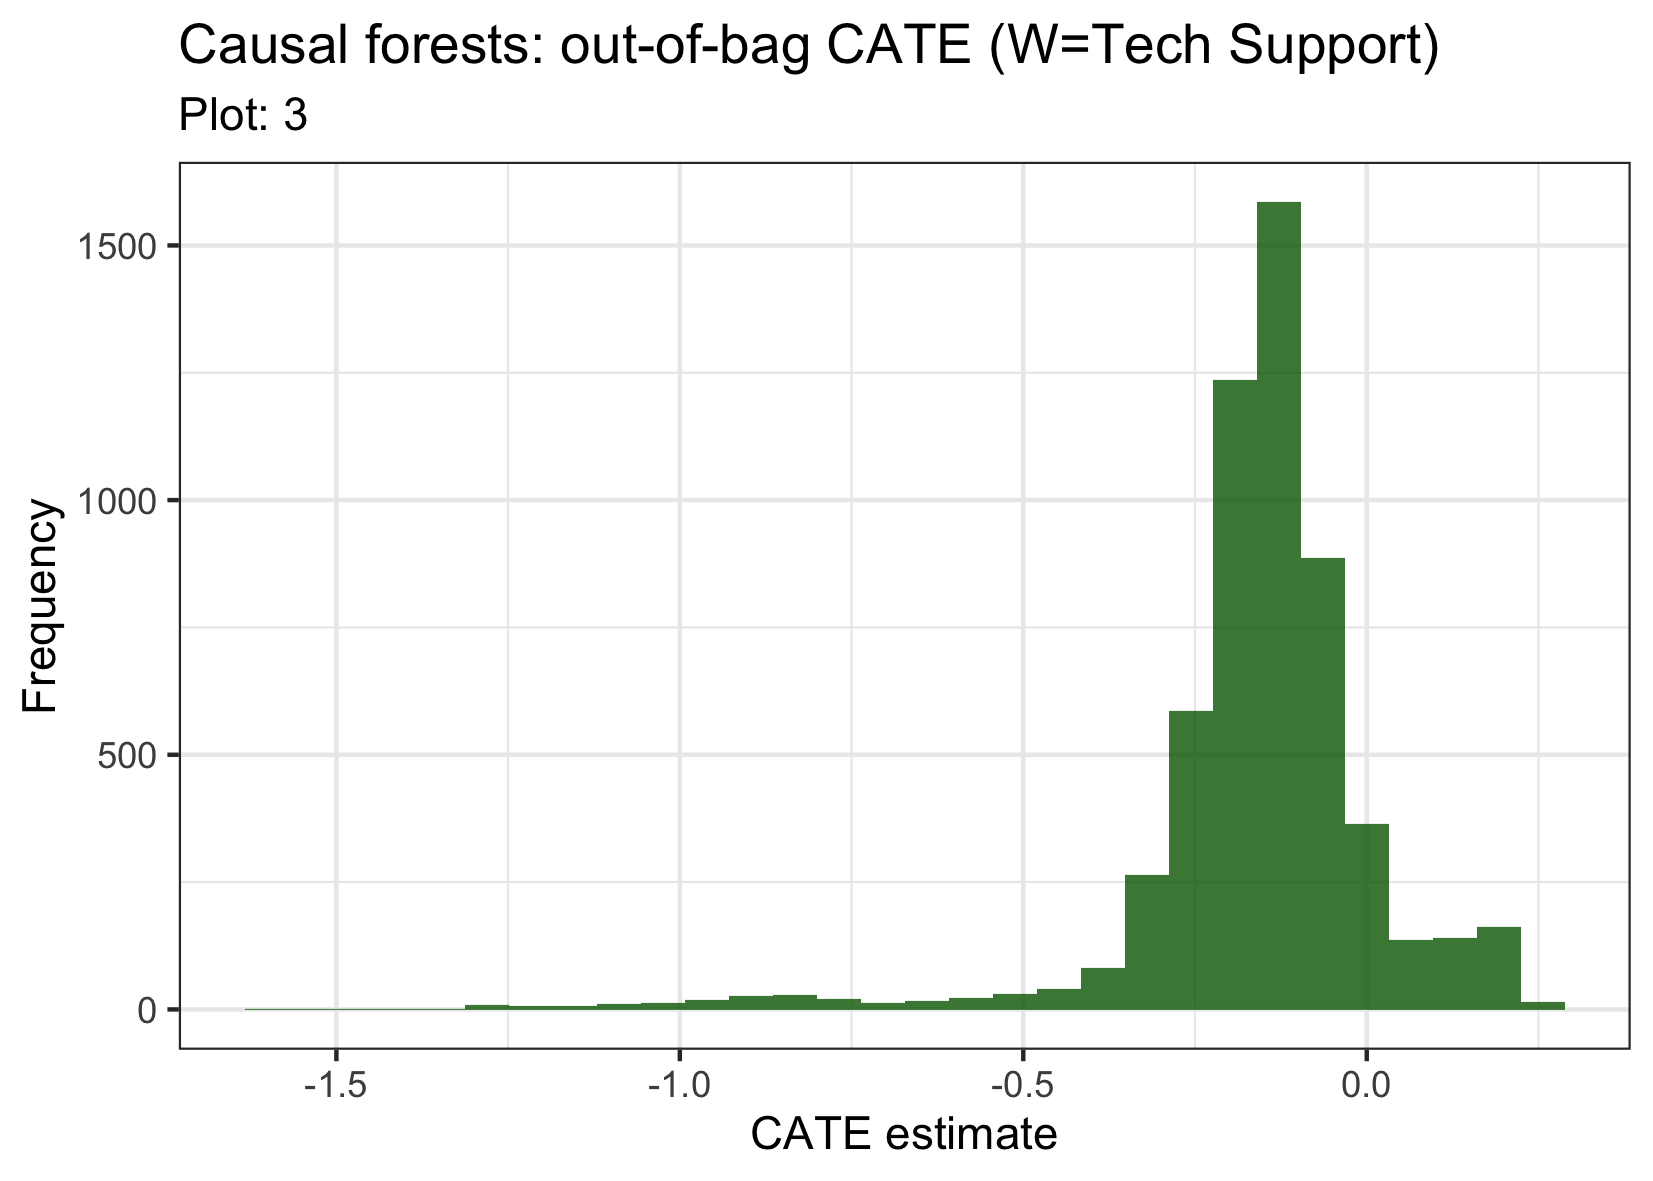
\includegraphics[scale=0.15]{chinchilab-template/chapters/appendices/ANALYSIS/CATE_3.png}
    \caption{Distribution of CATE (Model 3)}
    \label{fig:my_label}
\end{figure}

%%%%%%%%%%%%%%%%%%%%%%%%%%%%%%%%%%%%%%%%%%%%%%%%%%%%%%%%%%%%
\subsubsection{B.2.1.1 Nuisance Parameter Check}
%%%%%%%%%%%%%%%%%%%%%%%%%%%%%%%%%%%%%%%%%%%%%%%%%%%%%%%%%%%%
\begin{table}[H]{
    \begin{subtable}{.5\textwidth}
    \centering
    \scriptsize
        {\begin{tabular}{@{\extracolsep{5pt}}lc} 
        \\[-1.8ex]\hline 
        \hline \\[-1.8ex] 
         & \multicolumn{1}{c}{\textit{Dependent variable: Green Flag}} \\ 
        \cline{2-2} 
        \\[-1.8ex] &   \\ 
        \hline \\[-1.8ex] 
         e.bar & 1.002$^{***}$ \\ 
          & (0.029) \\ 
          & \\ 
         e.residual & 1.139$^{***}$ \\ 
          & (0.035) \\ 
          & \\ 
        \hline \\[-1.8ex] 
        \hline 
        \hline \\[-1.8ex] 
        \textit{Note:}  & \multicolumn{1}{r}{$^{*}$p$<$0.1; $^{**}$p$<$0.05; $^{***}$p$<$0.01} \\ 
        \end{tabular} }
    \subcaption{Outcome Model}
    \end{subtable}
    \begin{subtable}{0.3\linewidth}
    \centering
    \scriptsize
        {\begin{tabular}{@{\extracolsep{5pt}}lc} 
        \\[-1.8ex]\hline 
        \hline \\[-1.8ex] 
         & \multicolumn{1}{c}{\textit{Dependent variable: Green Flag}} \\ 
        \cline{2-2} 
        \\[-1.8ex] &   \\ 
        \hline \\[-1.8ex] 
         m.bar & 1.001$^{***}$ \\ 
          & (0.010) \\ 
          & \\ 
         m.residual & 1.206$^{***}$ \\ 
          & (0.014) \\ 
          & \\ 
        \hline \\[-1.8ex] 
        \hline 
        \hline \\[-1.8ex] 
        \textit{Note:}  & \multicolumn{1}{r}{$^{*}$p$<$0.1; $^{**}$p$<$0.05; $^{***}$p$<$0.01} \\ 
        \end{tabular} }
    \subcaption{Propensity Model}
    \end{subtable}
\caption{Calibration Regressions (Model 3)}
\label{x}}
\end{table}

\begin{figure}[h!]
    \centering
    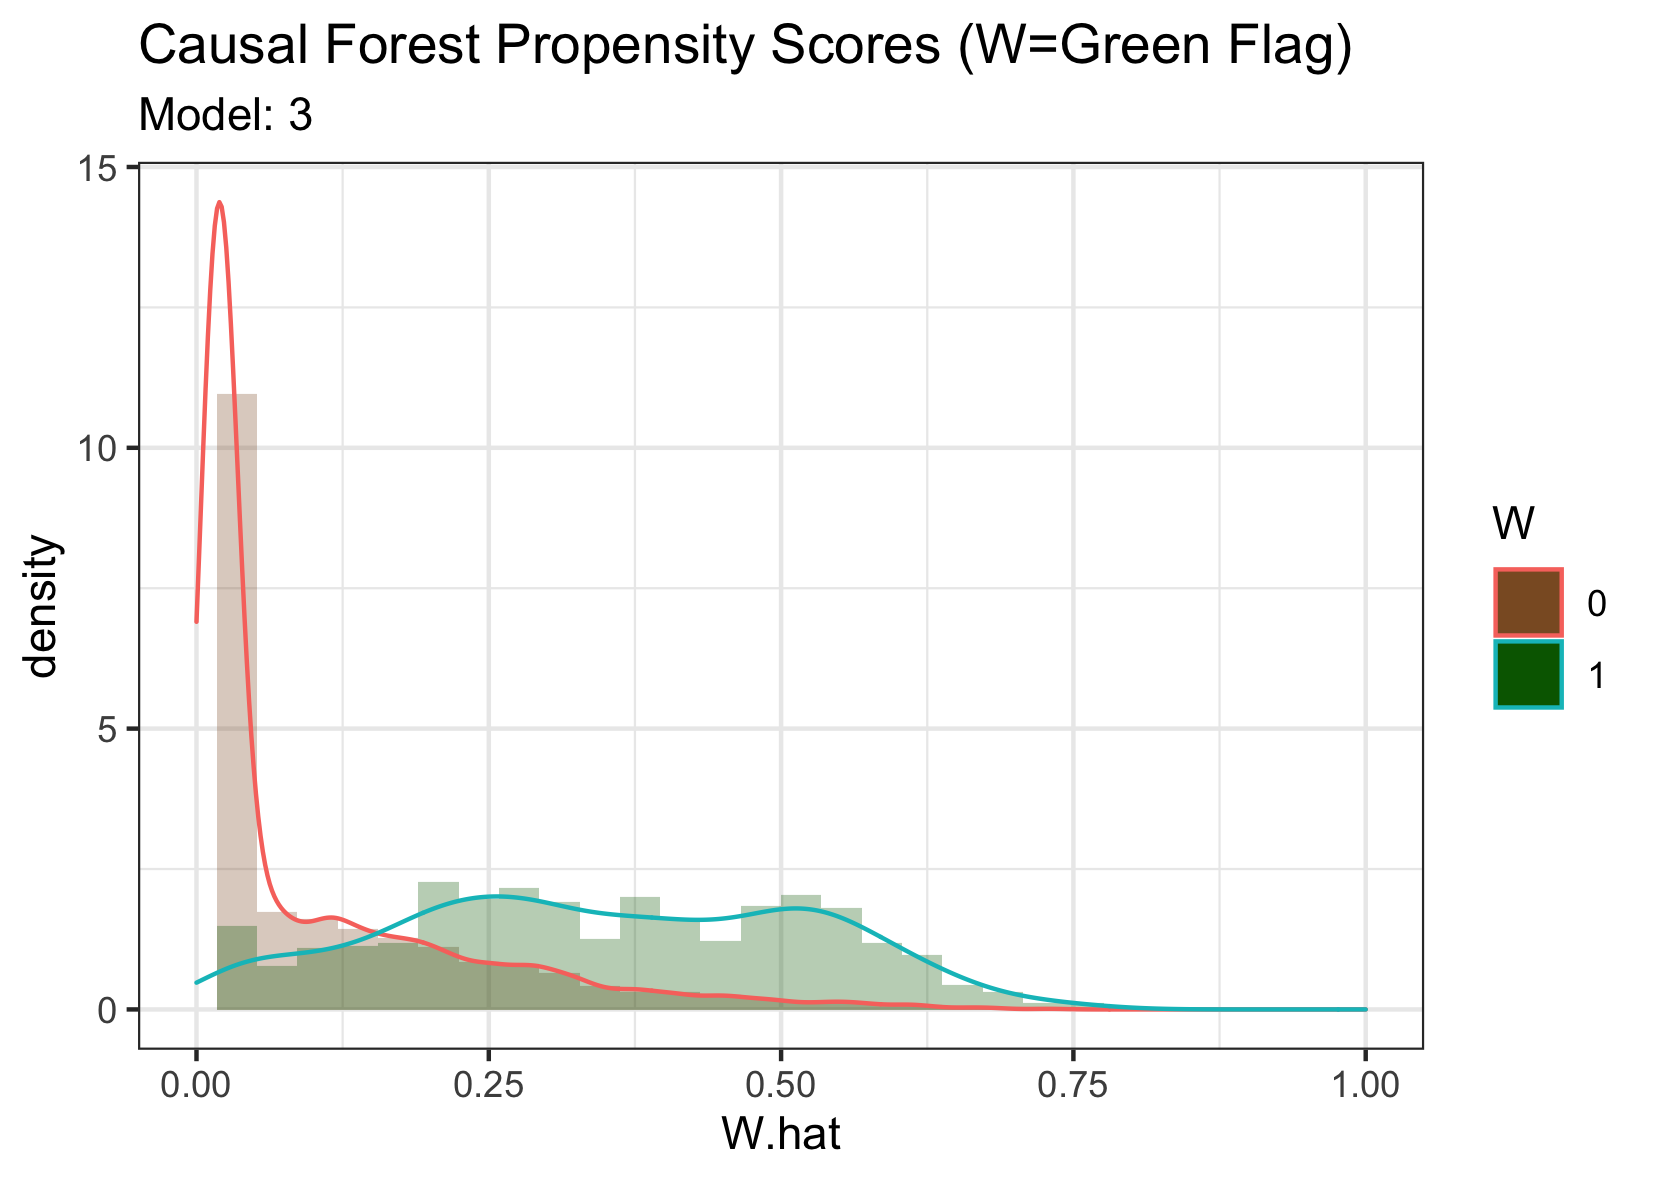
\includegraphics[scale=0.15]{chinchilab-template/chapters/appendices/ANALYSIS/prop_3.png}
    \caption{Propensity Score Distribution (Model 3)}
    \label{fig:my_label}
\end{figure}

%%%%%%%%%%%%%%%%%%%%%%%%%%%%%%%%%%%%%%%%%%%%%%%%%%%%%%%%%%%%
\subsubsection{B.2.1.2 Heterogeneity Assessment}
%%%%%%%%%%%%%%%%%%%%%%%%%%%%%%%%%%%%%%%%%%%%%%%%%%%%%%%%%%%%
\begin{table}[h!]
\centering
\caption{Variable Importance (Model 3)}
\begin{tabular}{lr}
\\[-1.8ex]\hline 
\hline \\[-1.8ex] 
\rowcolor[HTML]{FFFFFF} 
{\color[HTML]{333333} \textbf{Covariate}} & {\color[HTML]{333333} \textbf{Value}} \\ \hline
\rowcolor[HTML]{FFFFFF} 
{\color[HTML]{333333} 2022} & \cellcolor[HTML]{00441B}{\color[HTML]{FFFFFF} 0.23194018} \\
\rowcolor[HTML]{FFFFFF} 
{\color[HTML]{333333} Issue Amount} & \cellcolor[HTML]{005B25}{\color[HTML]{FFFFFF} 0.21746960} \\
\rowcolor[HTML]{FFFFFF} 
{\color[HTML]{333333} Time to Maturity (Days)} & \cellcolor[HTML]{1A823D}{\color[HTML]{FFFFFF} 0.18983740} \\
\rowcolor[HTML]{FFFFFF} 
{\color[HTML]{333333} 2021} & \cellcolor[HTML]{D5EFCF}{\color[HTML]{333333} 0.07048934} \\
\rowcolor[HTML]{FFFFFF} 
{\color[HTML]{333333} 2020} & \cellcolor[HTML]{E5F5E0}{\color[HTML]{333333} 0.05790504} \\
\rowcolor[HTML]{FFFFFF} 
{\color[HTML]{333333} A} & \cellcolor[HTML]{F7FCF5}{\color[HTML]{333333} 0.03261894} \\ \hline
\end{tabular}
\end{table}

\begin{figure}[h!]
    \centering
    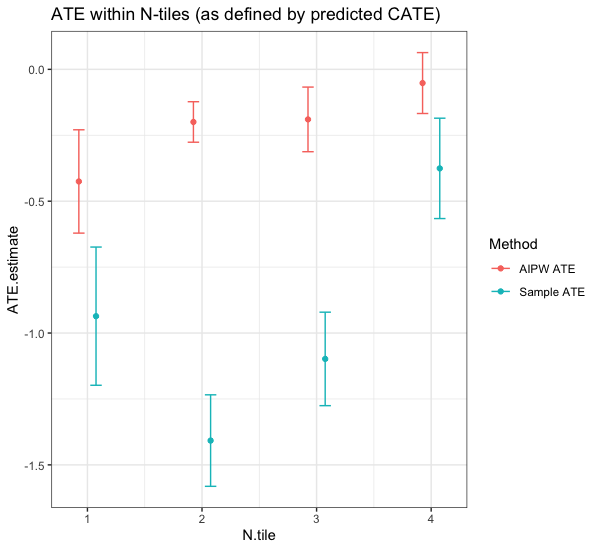
\includegraphics[scale=0.4]{chinchilab-template/chapters/appendices/ANALYSIS/ntile_cf1.png}
    \caption{Graph of ATE within Subgroups (Model 3)}
    \label{fig:my_label}
\end{figure}

\begin{figure}[H]
\centering
   \begin{subfigure}[b]{0.45\textwidth}
    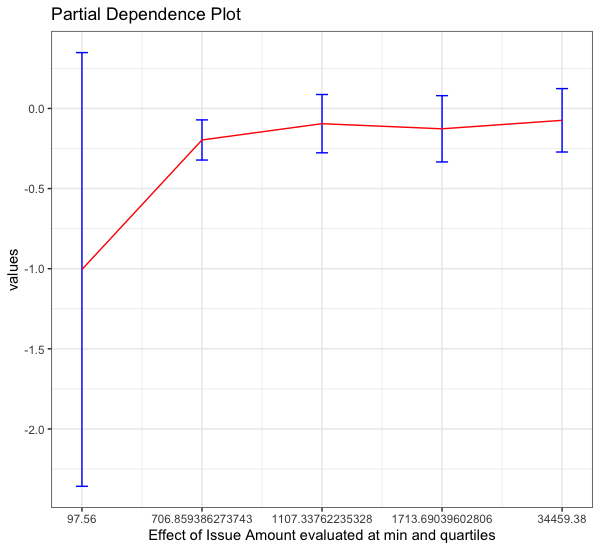
\includegraphics[width=0.8\textwidth]{chinchilab-template/chapters/appendices/ANALYSIS/PDP_cf1.png}
    \caption{Effect of Issue Amount}
   \label{fig:Ng1} 
\end{subfigure}
\begin{subfigure}[b]{0.4\textwidth}
    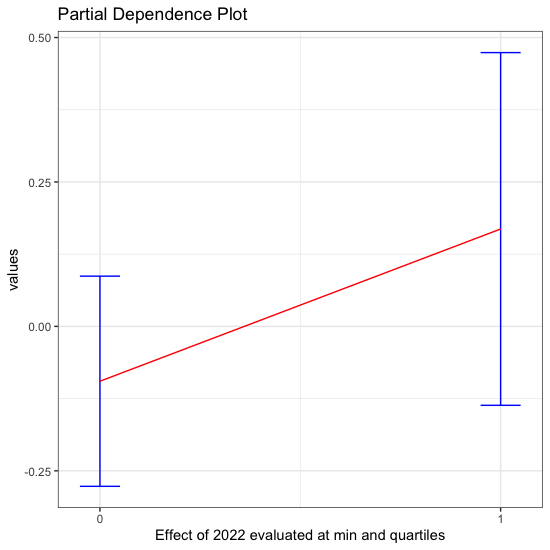
\includegraphics[width=0.8\textwidth]{chinchilab-template/chapters/appendices/ANALYSIS/PDP2_cf1.png}
    \caption{Effect of 2022}
   \label{fig:Ng2}
\end{subfigure}
\\
\begin{subfigure}[b]{0.45\textwidth}
    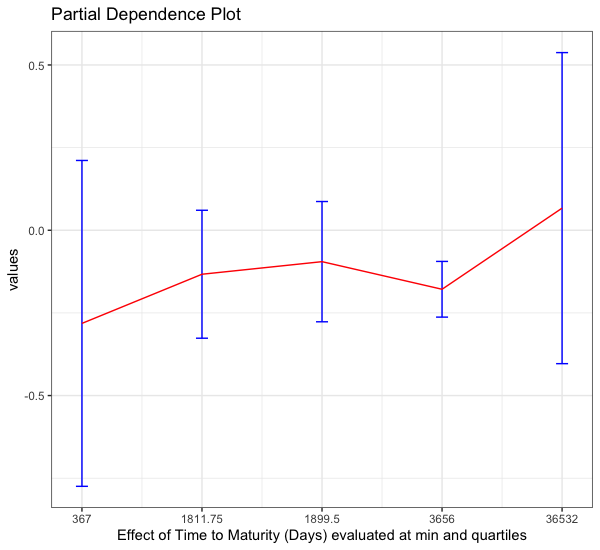
\includegraphics[width=0.8\textwidth]{chinchilab-template/chapters/appendices/ANALYSIS/PDP3_cf1.png}
    \caption{Effect of Time to Maturity (Days)}
   \label{fig:Ng2}
\end{subfigure}
\caption{Partial Dependency Plots (Model 3)}
\end{figure}

\newpage
